\section{Detailed Observation on LLM's Rationality}
\label{sec:observation}
This section provides an additional, comprehensive analysis of the rationality exhibited by LLM-based agents from various perspectives. Using Claude-3 Opus as a representative example, we examine the rational decision-making capabilities of LLMs in single-stage games through the following aspects:

\begin{enumerate}
    \item Consistency of action choices across variations in payoff matrices: By analyzing the agents' decisions in different payoff matrix scenarios, we can determine whether the LLM-based agents maintain consistent action choices or if their choices are influenced by nuanced changes in the payoff matrix.
    \item Consistency of action choices across designated personalities in system prompts: We investigate the impact of assigned personalities in system prompts on the agents' decision-making process. This analysis helps us understand whether the LLM-based agents' rationality is affected by the designated personality or if they maintain consistent action choices regardless.
    \item Maintenance of rationality under discussion and multi-round discussions: We explore how the agents' rationality evolves when engaged in discussions or multi-round interactions. This examination reveals whether the LLM-based agents can maintain their rationality or if it is influenced by the communication and negotiation processes.
\end{enumerate}

\subsection{Experiment Setup}
In each experimental setup, we conduct 10 iterations utilizing a temperature value of 1 for the Claude-3 model. Each player within these setups is represented by an LLM-based agent. For each configuration, we document the probability distribution of the actions executed by these agents.

\subsection{Variance of Payoff Matrix}
\begin{definition}[Nash-Equilibrium invariant perturbation]
A Nash Equilibrium Invariant Perturbation is a modification to the numerical values within a game's payoff matrix that preserves the set of Nash equilibria. Formally, consider a finite game $G = (N, \{S_o\}_{i\in N}, \{\pi_i\}_{i\in N})$ where $N$ is the set of players, $S_i$ is the strategy set for player $i$, $\pi_i: S\to\mathcal{R}$ is the payoff function for player $i$.

A perturbed game $G' = (N, \{S_i\}_{i\in N}, \{\pi_i'\}_{i\in N})$ of the game $G$ is defined by adjusted payoff functions $\pi_i' = \pi_i + \delta_i$ where $\delta_i: S\to \mathcal{R}$ represnts the change in payoffs for player $i$. The perturbation $\delta = \{\delta_i\}_{i\in N}$ is termed a Nash Equilibrium Invariant Perturbation if the set of Nash equilibria remains unchanged between the original game $G$ and the perturbed game $G'$.
\end{definition}

Traditional evaluation of LLM on rationality utilize traditional game-theoretic scenarios. If LLMs do have rationality, then their rationality should be consistent across different instantiation of the payoff matrix. 

To study this, we use the traditional game of Prisoner's Dilemma and Stag Hunt.


We introduce certain modifications to the traditional payoff matrices while ensuring that the rational choices remain unaltered. Despite these variations, the Nash Equilibrium remains consistent across all modifications. Consequently, if an agent is rational, it is expected to make the same rational choices in each scenario. We present the variations here:


\begin{table}[htb]%\[!htb\]
\centering
\setlength{\tabcolsep}{10pt}
    \begin{subtable}[t]{.48\textwidth}
        \centering
        \captionsetup{labelformat=empty}
            \begin{tabular}{l|cc}
                 & action 1 & action 2 \\
                \toprule
                action 1 & 300, 300 & 0, 301  \\
                action 2 & 301, 0\phantom{00} & 1, 1\phantom{01}  \\
            \end{tabular}
        \caption{Table \thetable \alph{subtable}: Variation 1: payoff matrix for Prisoner's Dilemma}
    \end{subtable}%
    \hfill
   \begin{subtable}[t]{.48\textwidth}
        \centering
        \captionsetup{labelformat=empty}
        \begin{tabular}{l|cc}
                 & action 1 & action 2 \\
                \toprule
                action 1 & 3, \phantom{-}3\phantom{00} & -300, \phantom{-}5\phantom{00} \\
                action 2 & 5, -300 & -299, -299  \\
            \end{tabular}
        \caption{Table \thetable \alph{subtable}: Variation 2: payoff matrix for Prisoner's Dilemma}
    \end{subtable}
\end{table}

\begin{table}[htb]%\[!htb\]
\centering
\setlength{\tabcolsep}{10pt}
    \begin{subtable}[t]{.48\textwidth}
        \centering
        \captionsetup{labelformat=empty}
            \begin{tabular}{l|cc}
                 & action 1 & action 2 \\
                \toprule
                action 1 & 300, 300 & 0, 1  \\
                action 2 & \phantom{30}1, 0\phantom{00} & 1, 1  \\
            \end{tabular}
        \caption{Table \thetable \alph{subtable}: Variation 1: payoff matrix for Stag Hunt}
    \end{subtable}%
    \hfill
   \begin{subtable}[t]{.48\textwidth}
        \centering
        \captionsetup{labelformat=empty}
        \begin{tabular}{l|cc}
                 & action 1 & action 2 \\
                \toprule
                action 1 & \phantom{-9}3, \phantom{-}3\phantom{00} & -100, -99 \\
                action 2 & -99, -100 & \phantom{0}-99, -99  \\
            \end{tabular}
        \caption{Table \thetable \alph{subtable}: Variation 2: payoff matrix for Stag Hunt}
    \end{subtable}
\end{table}

% \begin{figure}[!ht]
%     \centering
%     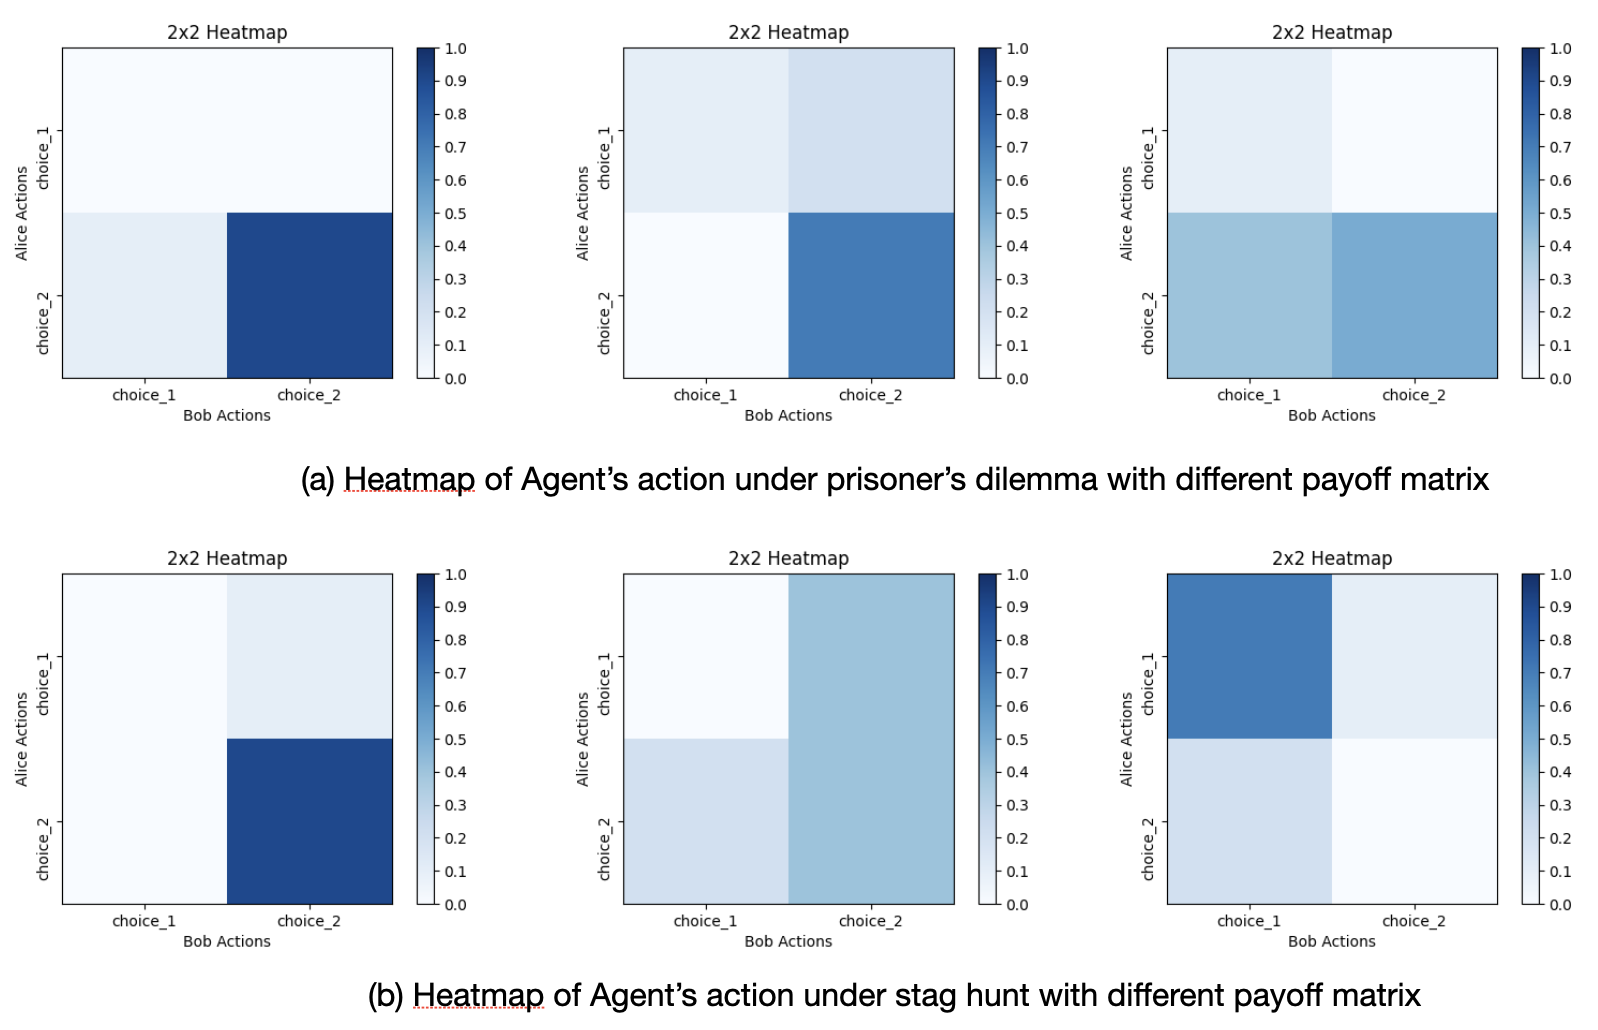
\includegraphics[scale=0.5]{Fig/payoff.png}
%     \vspace{5pt}\caption{Agents' performance under different payoff matrix}
%     \label{fig:payoff}
% \end{figure}

\begin{figure}[!ht]
    \hspace*{-2cm}
    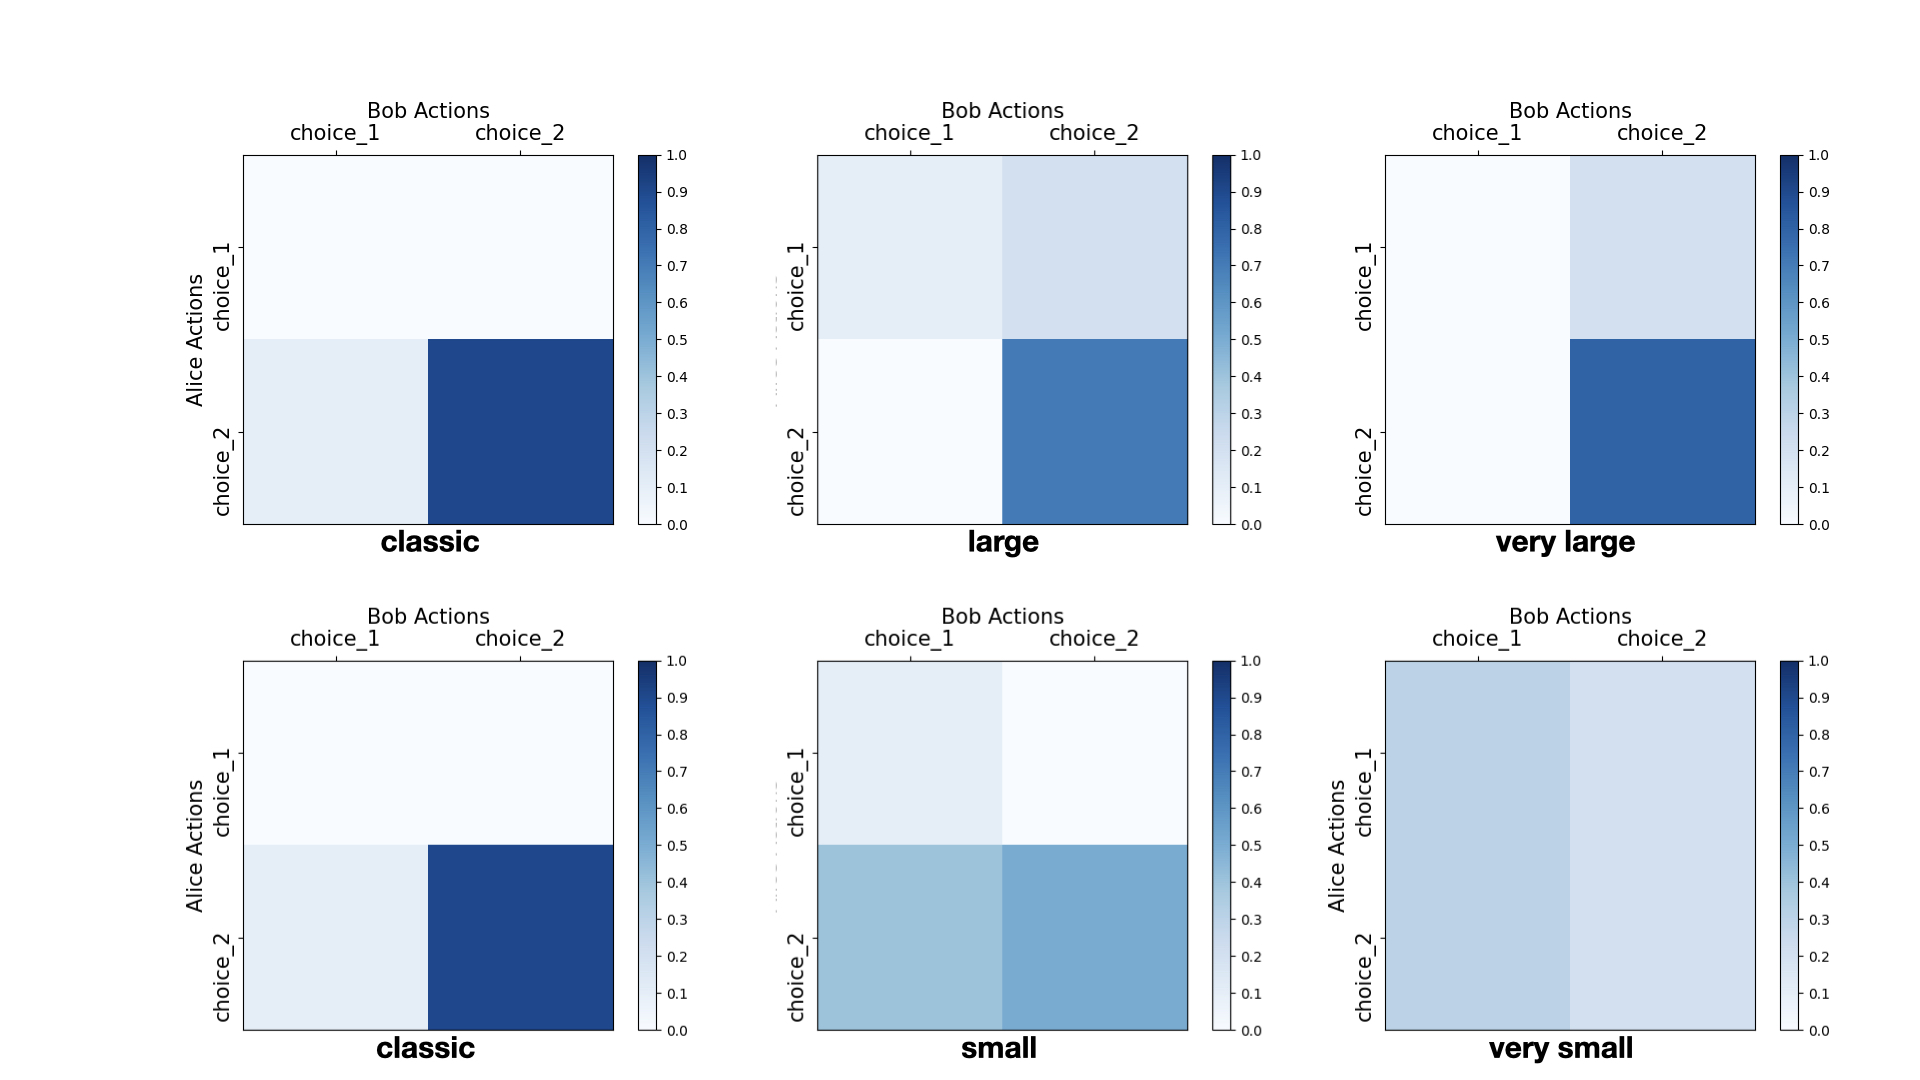
\includegraphics[scale=0.25]{Fig/payoff_pd.jpeg}
    \caption{Agents' performance under different payoff matrix for Prisoner's Dilemma}
    \label{fig:payoff_pd}
\end{figure}

\begin{figure}[!ht]
    \hspace*{-2cm}
    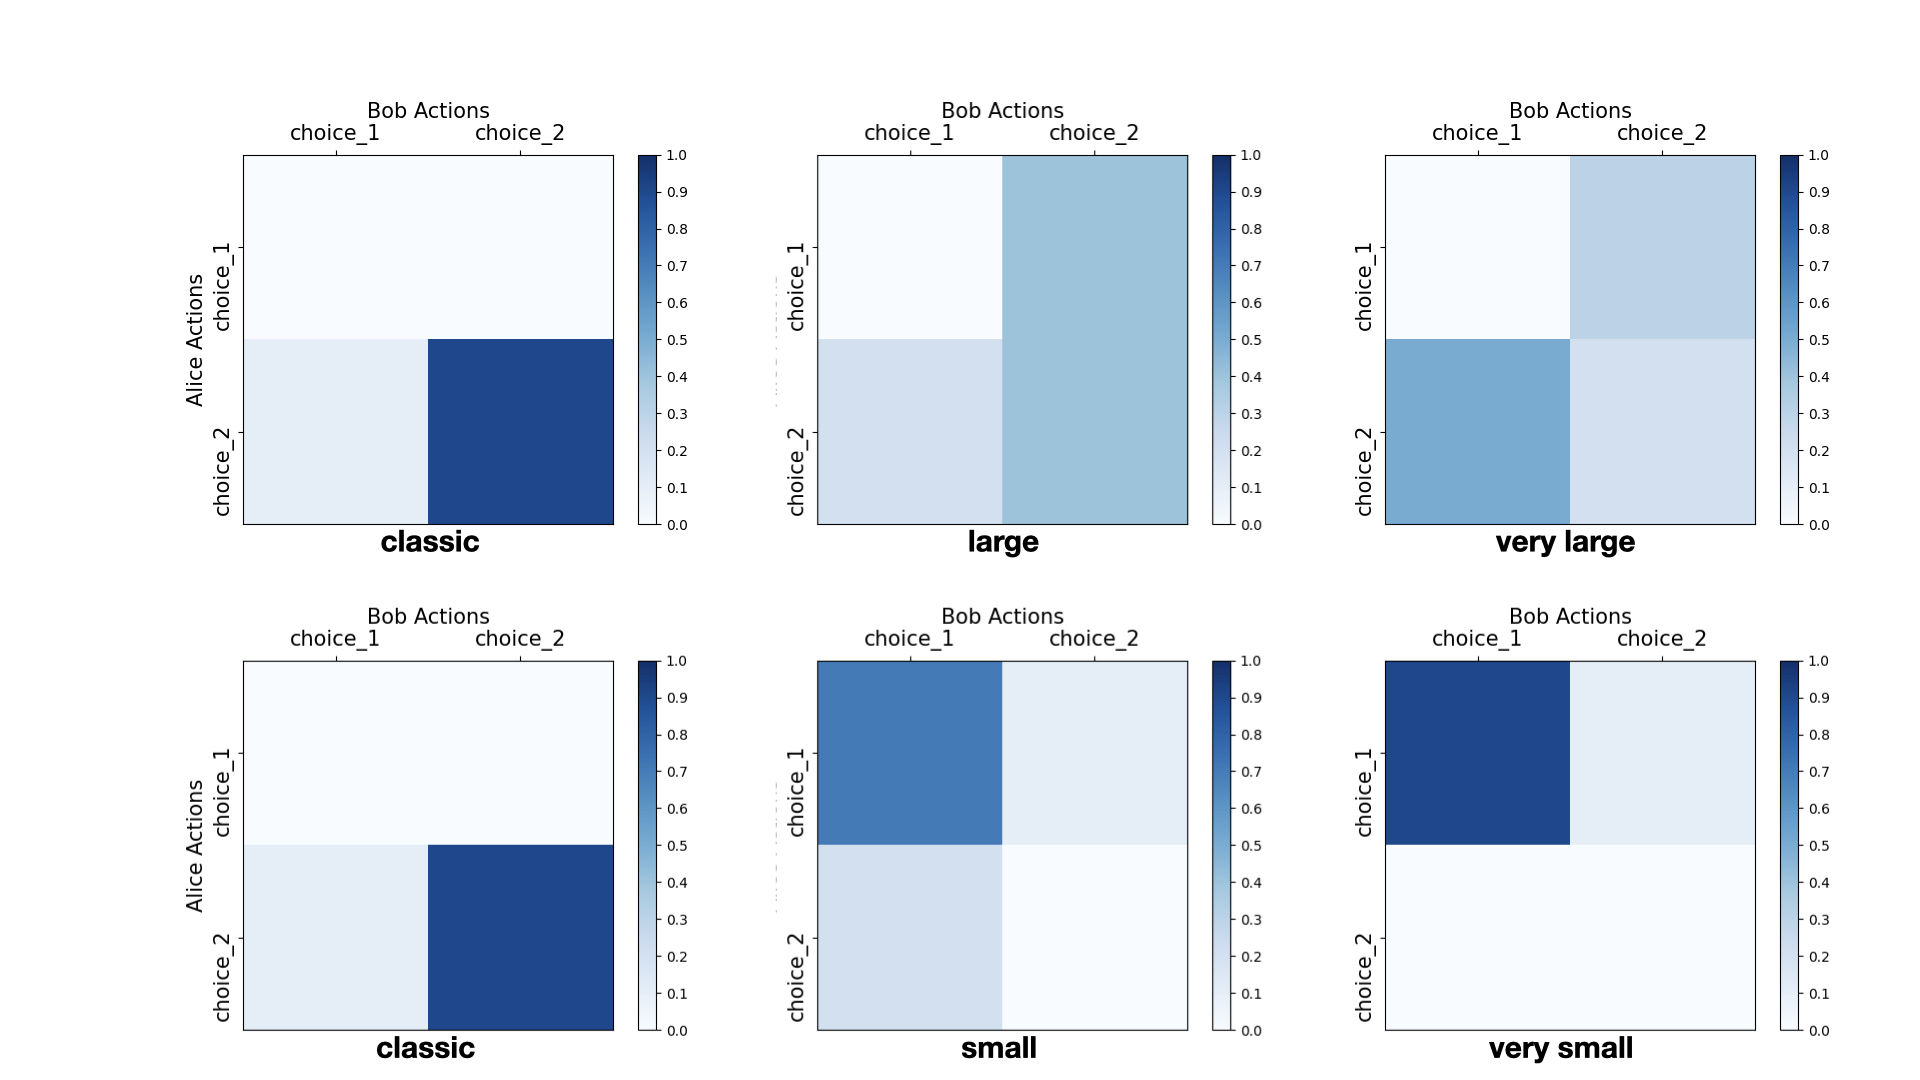
\includegraphics[scale=0.25]{Fig/payoff_sh.jpeg}
    \caption{Agents' performance under different payoff matrix for Stag Hunt}
    \label{fig:payoff_sh}
\end{figure}

We conduct experiments on these two games with their variations. Figures~\ref{fig:payoff_pd} and~\ref{fig:payoff_sh} contain experiment results of the action distribution. Contrary to the expectation that performance should remain unaffected by payoff variations, the results demonstrate inconsistent performance distribution across different payoff scenarios. In the case of Prisoner's Dilemma, the probability of the rational situation (Action 2, Action 2) is significantly higher in the classic payoff matrix but considerably lower in the two variations. Similarly, in Stag Hunt, the actions taken also vary across different payoff scenarios. These findings suggest that the LLMs are either (1) not consistently making rational decisions or (2) their rationality is heavily influenced by other irrational factors.

\subsection{Variation of Personality}
In addition to investigating the impact of payoff variations on the rationality of agents, we also examine whether the personality denoted in the system prompt influences the agents' rationality. If the agents are consistent in their computation and calculation of the reward, then their rationality should not be affected by the assigned ``personality''. The system prompt template used for this experiment is as follows:

\begin{verbatim}
You are a {{personality}} assistant that carefully answer the question.
\end{verbatim}

For the personality variable, we select six different but common adjectives: compassionate, friendly, helpful, pragmatic, rational, and witty. The results of this experiment are presented in Figure 
\ref{fig:personality}. The findings indicate that the agents' performance varies significantly according to the assigned personality. The ``witty'' personality yields the game-theoretically most rational option, while the ``rational'' personality performs slightly worse. For other personalities, such as ``compassionate'', ``friendly'', ``helpful'', and ``pragmatic'', the agents exhibit decreased rationality and frequently make irrational choices.


\begin{figure}[!ht]
    \hspace*{-2cm}
    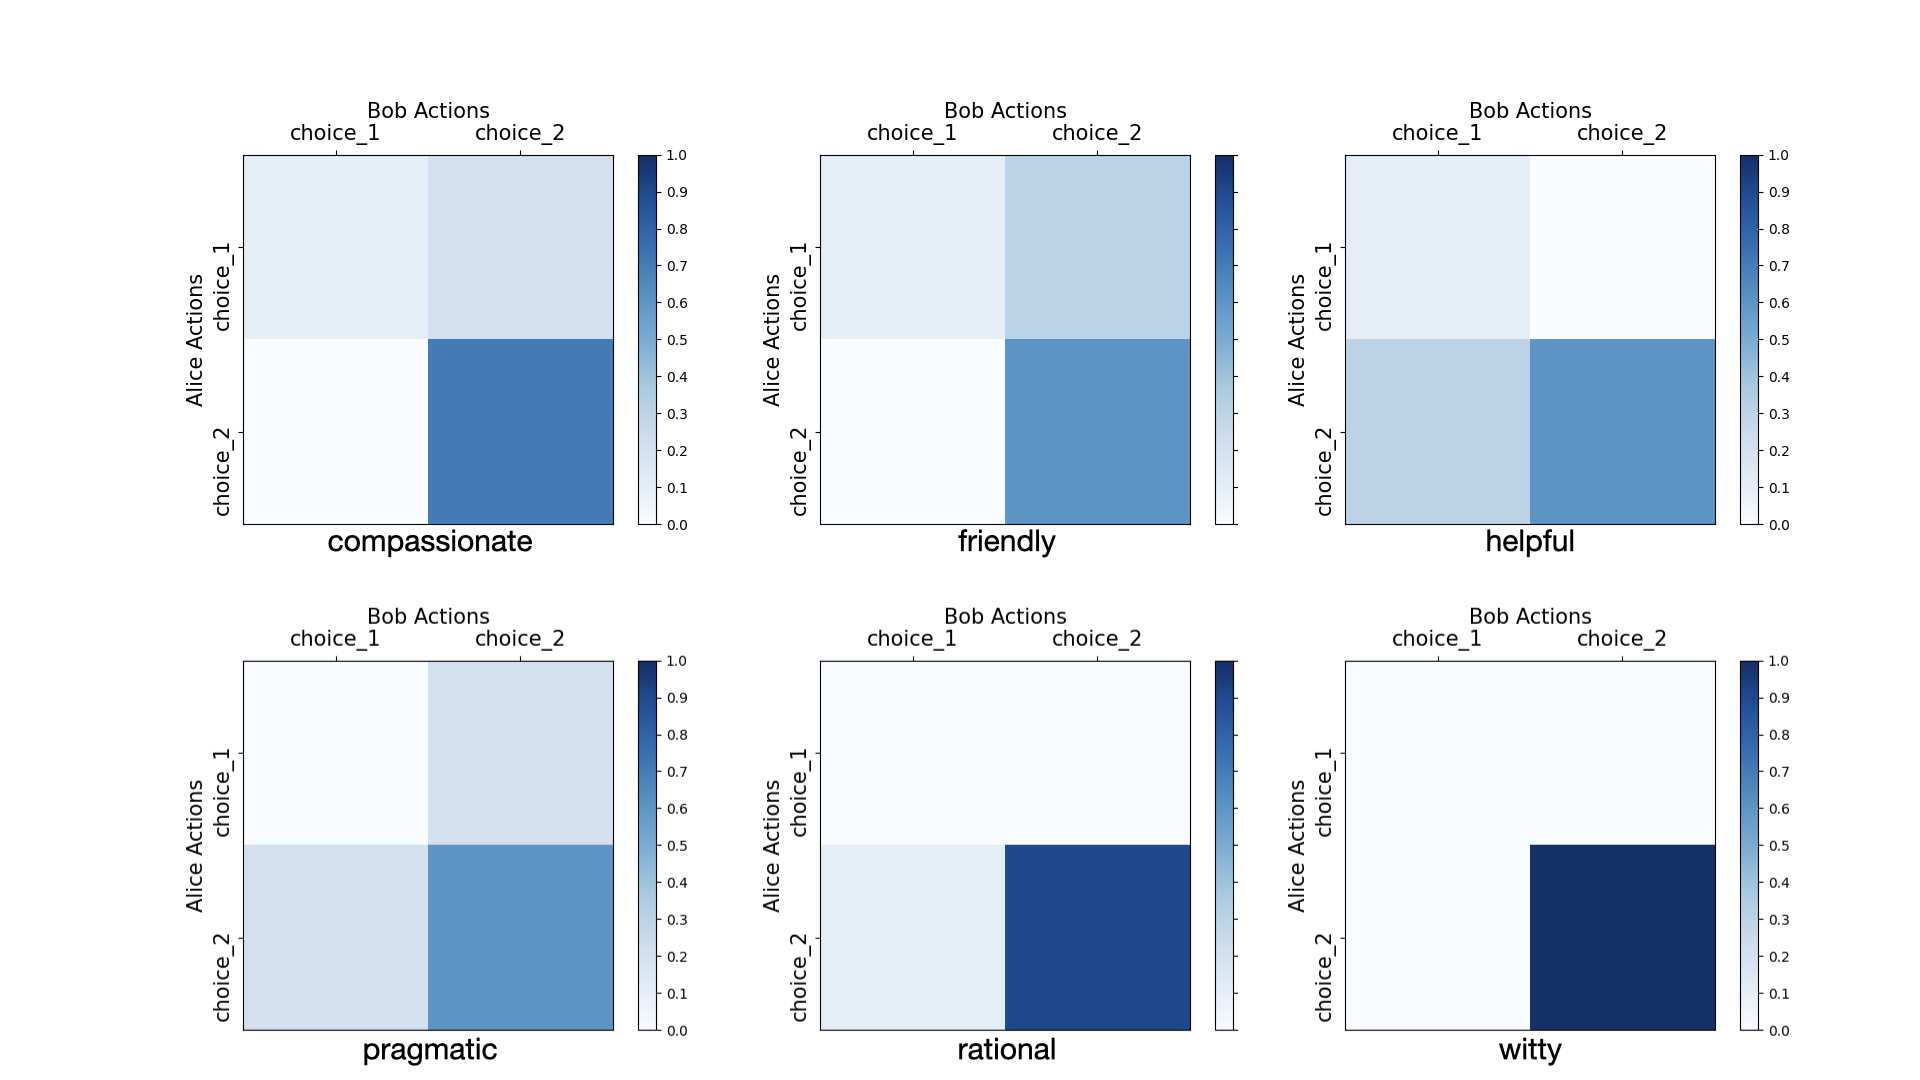
\includegraphics[scale=0.25]{Fig/personality.jpeg}
    \vspace{5pt}\caption{Agents' performance under different system prompt with personality}
    \label{fig:personality}
\end{figure}


\subsection{Does negotiation affect rationality?}
In certain situations, the decision-making process of agents can be influenced by discussions with other agents. For instance, in the game of Stag Hunt, effective negotiation can foster trust between players, enabling them to recognize that individual efforts to capture a hare are not as advantageous as cooperating to hunt a stag. Consequently, successful communication should encourage players to select the pareto optimal Nash equilibrium instead of either of the two available equilibriums. However, there are scenarios where negotiation does not impact the outcome. In the case of Prisoner's Dilemma, communication fails to establish trust, as each player's dominant strategy is to defect regardless of the other player's action. Therefore, communication is unlikely to affect performance, as the rational choice remains unchanged. 

In our current experimentation, we focus on four game-theoretic scenarios: Stag Hunt, Battle of the Sexes, Prisoner's Dilemma, and Rock-Paper-Scissors. The impact of negotiation on these games varies as follows:
\begin{itemize}
    \item Stag Hunt: In this game, negotiation plays a significant role in achieving the pareto optimal rational choice. Effective communication between players can foster trust and encourage cooperation, leading to better outcomes for both parties.
    \item Battle of the Sexes: Negotiation is crucial for enhancing coordination between the two players in this game. By discussing their preferences and intentions, players can reach a more coherent and mutually beneficial strategy.
    \item Prisoner's Dilemma: The presence of a single Nash Equilibrium in this game renders negotiation irrelevant. Regardless of any discussion, the rational choice for both players remains the same, and the outcome is determined by their individual decisions.
\end{itemize}

To investigate the impact of communication on agents' choices, we conduct experiments on both games with and without communication. In the communication setup, agents are allowed to exchange messages before making decisions. We record the action distribution of agents in each setup and present the results in Figure~\ref{fig:negotiation_round} for 0, 1, and 2 rounds of negotiation.

\begin{figure}[!ht]
    \hspace*{-1cm}
    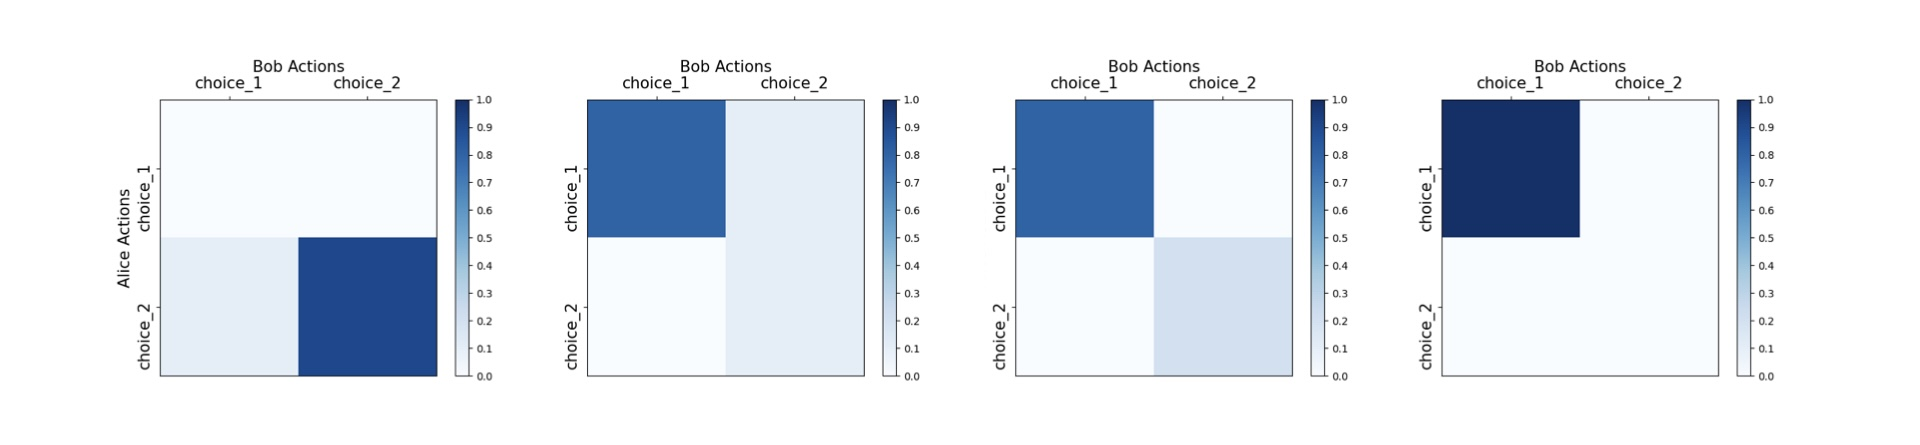
\includegraphics[scale=0.24]{Fig/negotiation_pd.jpeg}
    \hspace*{-1cm}
    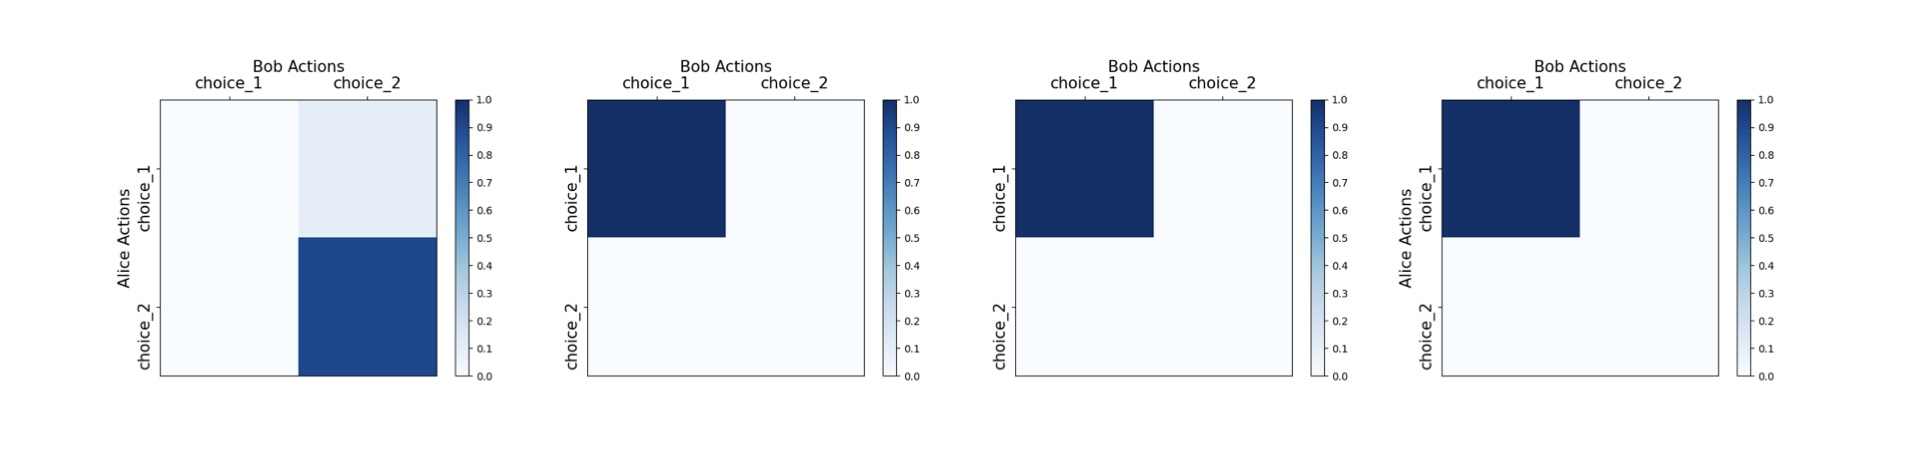
\includegraphics[scale=0.24]{Fig/negotiation_sh.jpg}
    \hspace*{-1cm}
    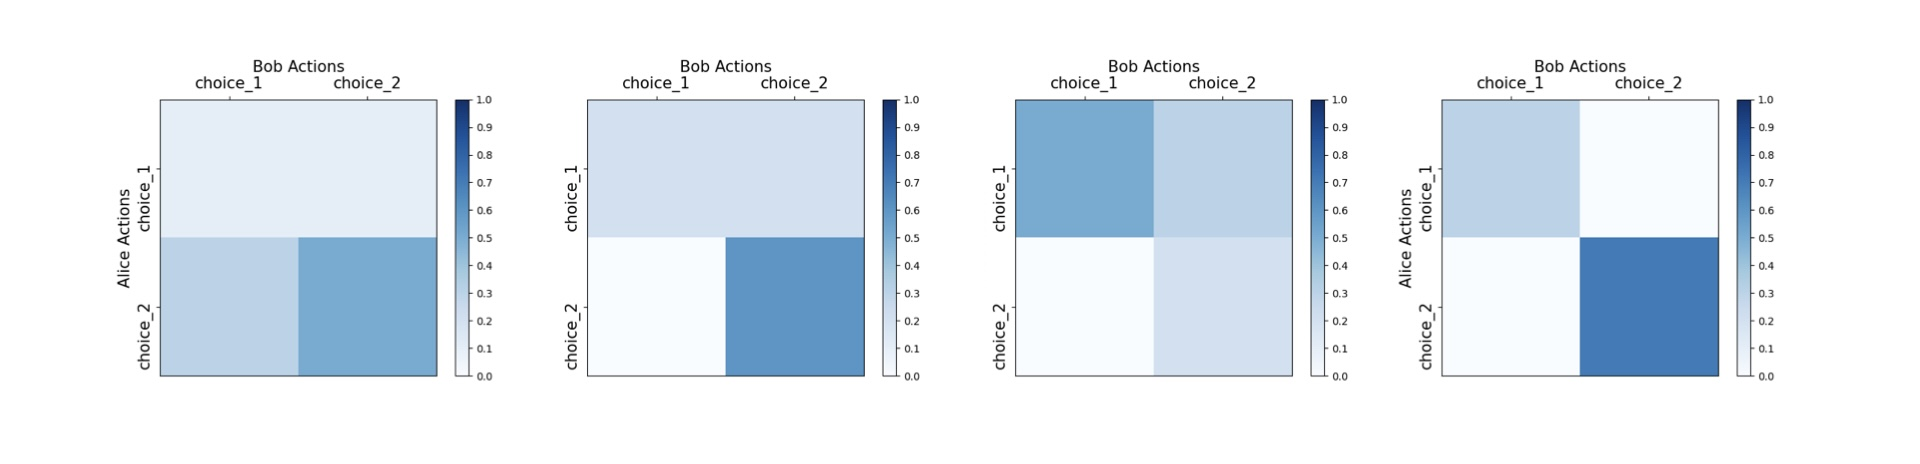
\includegraphics[scale=0.24]{Fig/negotiation_bs.jpg}
    \vspace{5pt}\caption{Agents' performance under different numbers of negotiation: 0-round, 1-round, 2-round, and 3-round from left to right for the four games}
    \label{fig:negotiation_round}
\end{figure}

Based on our observations, we have identified several inconsistencies between our expectations and the actual outcomes in the various game-theoretic scenarios:
\begin{itemize}
    \item Stag Hunt (Figure~\ref{fig:negotiation_round} (b)): As expected, negotiation leads to the adoption of the pareto optimal strategy. This result demonstrates that effective communication can facilitate cooperation and achieve better outcomes for all parties involved.
    \item Battle of the Sexes: (Figure~\ref{fig:negotiation_round} (c)): Our findings indicate an increase in coordination between players as the number of negotiation rounds increases. This outcome suggests that negotiation plays a crucial role in enhancing mutual understanding and promoting more coherent strategies.
    \item Prisoner's Dilemma (Figure~\ref{fig:negotiation_round} (a)): Contrary to expectations, players consistently gravitate towards the dominated strategy after negotiation. This result is surprising, as the presence of a single Nash Equilibrium should render negotiation irrelevant.
\end{itemize}

In summary, our findings suggest that negotiation does not always lead to the pareto optimal decision-making, and in some cases, it may even result in the loss of rationality. Further investigation is necessary to understand the underlying factors contributing to these unexpected outcomes.

\subsection{How does prompt affect the influence of negotiation?}
Some people may want to ask can we use simple prompt engineering to control the effect of negotiation. 

To investigate whether the observed negative impact of negotiation on player rationality can be mitigated through simple prompt engineering, we design six distinct prompts. The first three prompts emphasize caution regarding the other player's statements and encourage the agent to critically evaluate trustworthiness. These prompts are intended to foster a more skeptical and analytical mindset during negotiations.
The remaining three prompts are formulated as commands, instructing the agent to make decisions independently without being influenced by the negotiation process. The objective of these prompts is to promote autonomy and self-reliance in the agent's decision-making, potentially minimizing the negative effects of negotiation on rationality.

In our experiment, we incorporate the six designed prompts at the end of the entire action-making prompt for each game. This placement ensures that the prompts serve as a final reminder or instruction to the LLM-based agents, not affected by the length of the negotiation texts.

\begin{verbatim}
Prompt 1: Please carefully analyze the negotiation messages, think about 
whether you can trust the other player's message, and make your own decision.
\end{verbatim}

\begin{verbatim}
Prompt 2: Please carefully analyze the negotiation messages and make your own 
decision.
\end{verbatim}

\begin{verbatim}
Prompt 3: Carefully analyze and think about whether you can trust the other 
player's message, and then make your own decision.
\end{verbatim}

\begin{verbatim}
Prompt 4: You can choose your own choice regardless what the other player 
says.
\end{verbatim}

\begin{verbatim}
Prompt 5: You should make your own choice regardless what the other player 
says.
\end{verbatim}

\begin{verbatim}
Prompt 6: You must make your own choice regardless what the other player says.
\end{verbatim}


\begin{figure}[!ht]
    \hspace*{-1cm}
    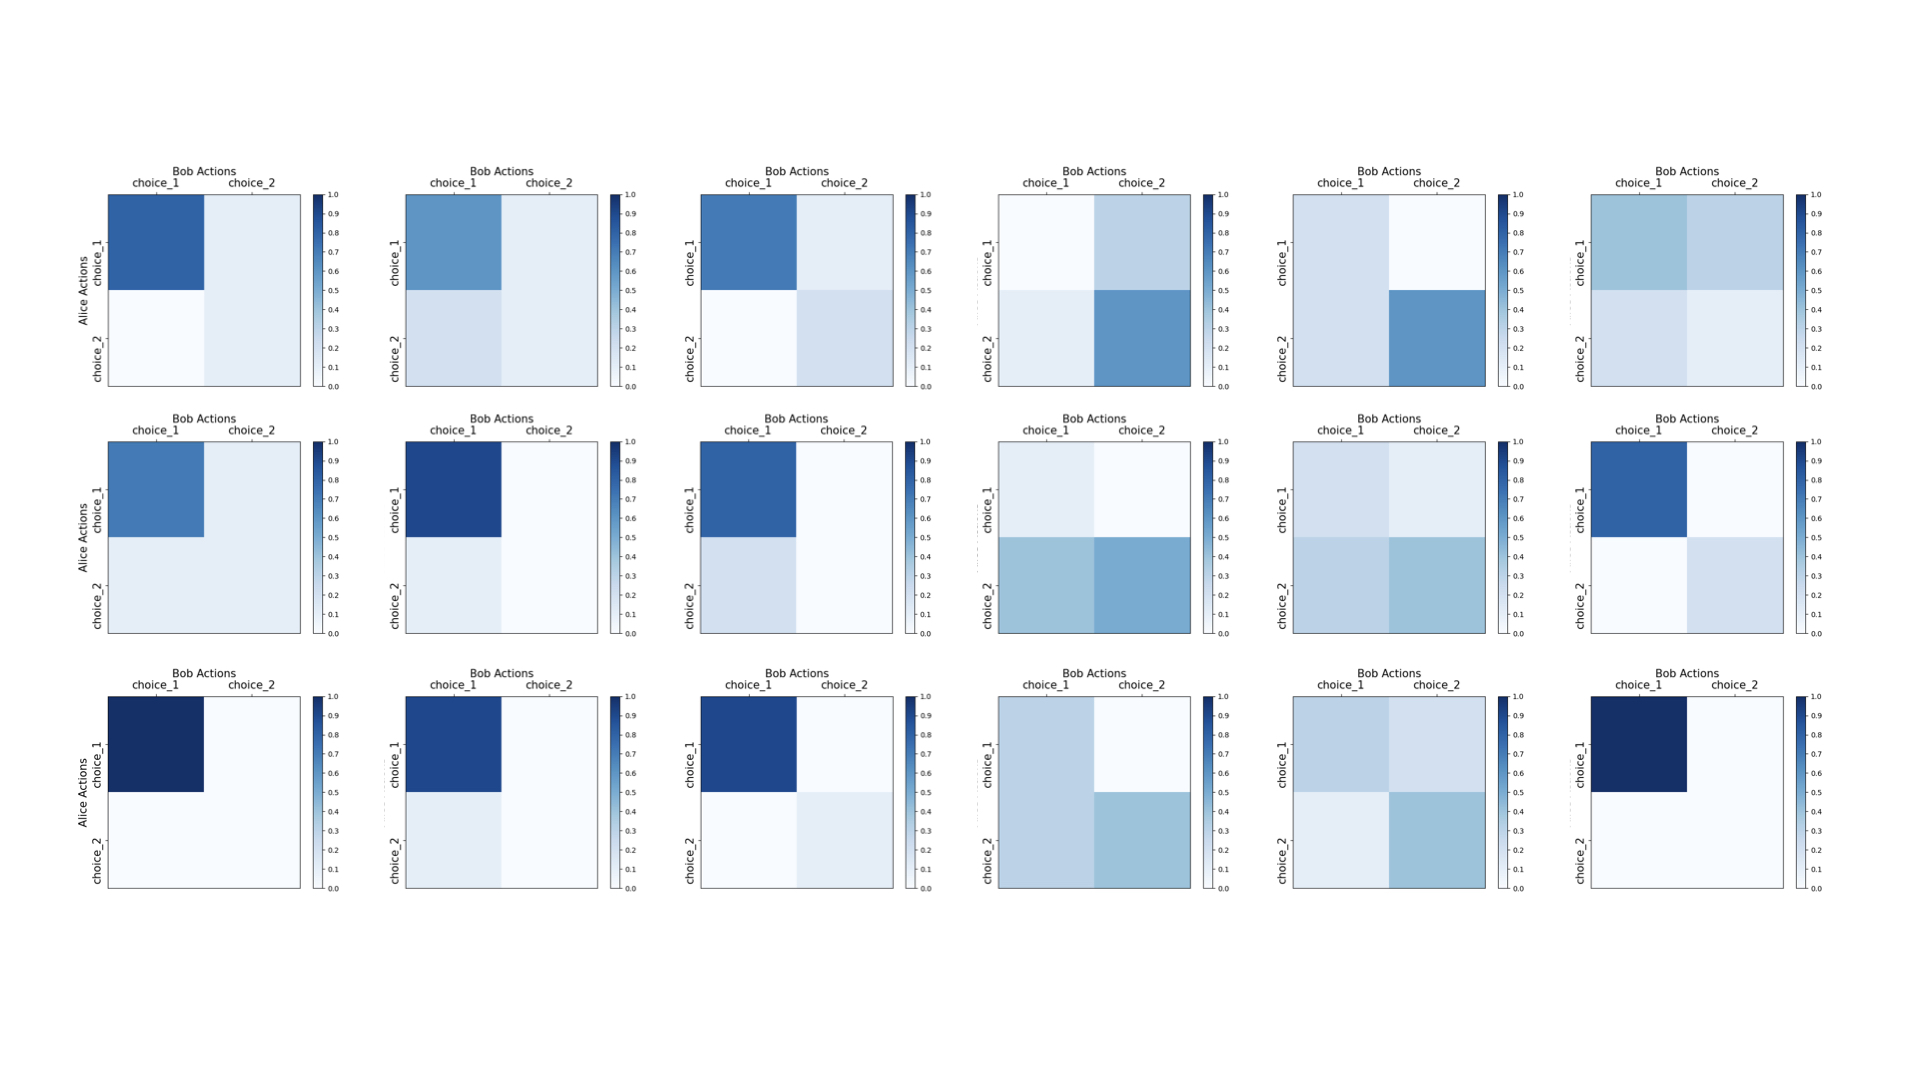
\includegraphics[scale=0.25]{Fig/negotiation_prompt_round_pd.jpeg}
    \caption{The effect of the 6 engineered prompts on Prisoner's Dilemma game with different rounds of negotiation: 1-round, 2-round, and 3-round for the three rows}
    \label{fig:negotion_prompt_on_round_pd}
\end{figure}

\begin{figure}[!ht]
    \hspace*{-1cm}
    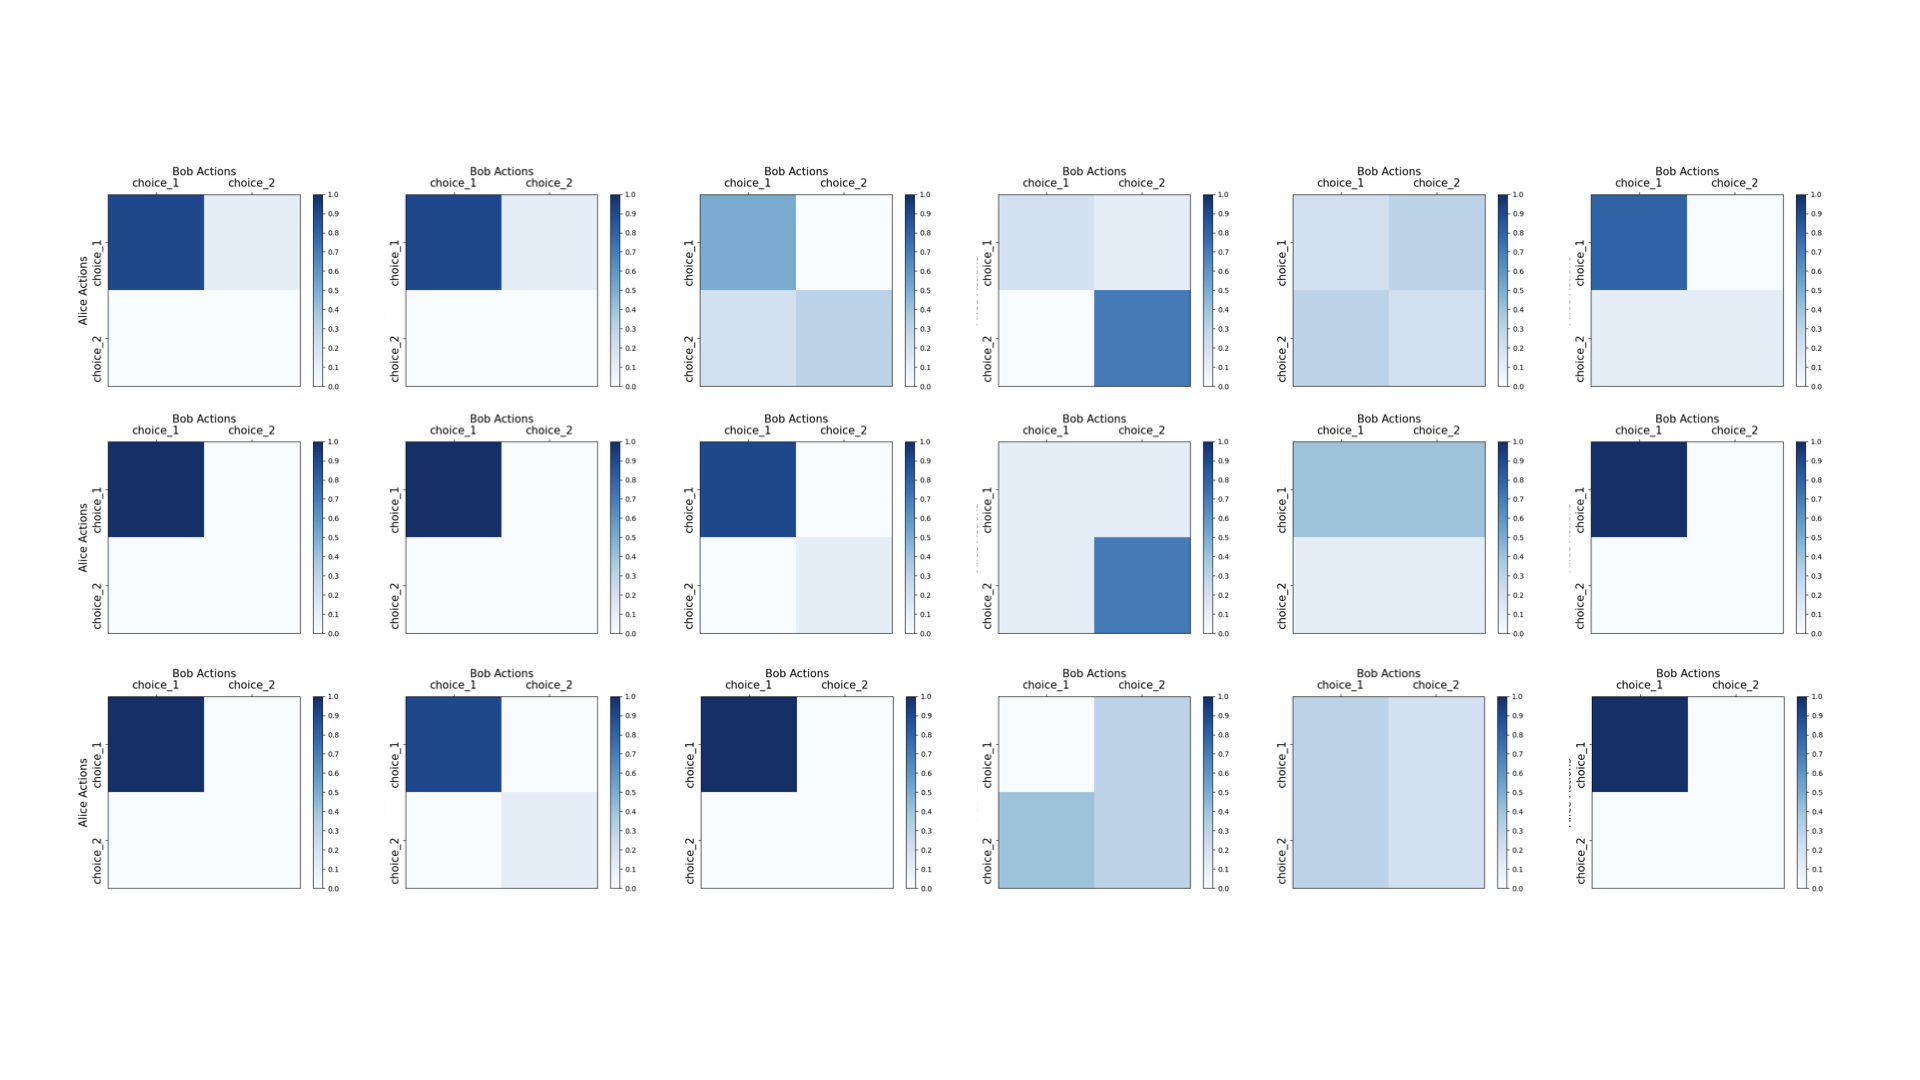
\includegraphics[scale=0.25]{Fig/negotiation_prompt_round_sh.jpeg}
    \caption{The effect of the 6 engineered prompts on Stag Hunt game with different rounds of negotiation: 1-round, 2-round, and 3-round for the three rows}
    \label{fig:negotion_prompt_on_round_sh}
\end{figure}


By comparing the performance of LLM-based agents across these six prompts, we aim to determine whether prompt engineering can effectively control the impact of negotiation on player rationality and improve decision-making outcomes in various game-theoretic scenarios. Figure~\ref{fig:negotion_prompt_on_round_sh} and Figure~\ref{fig:negotion_prompt_on_round_sh} illustrate the impact of the six designed prompts on the outcomes of Prisoner's Dilemma and Stag Hunt games, respectively. In each figure, the six columns correspond to the specific prompts used, while the three rows represent the number of negotiation rounds between the two players before they decide on their actions.

By analyzing these figures, we can assess the effectiveness of each prompt in influencing the players' decision-making processes and evaluate whether prompt engineering can mitigate the effects of negotiation on player's choices as the number of negotiation round increases.


In observation, we can see the following situations:
\begin{enumerate}
    \item Prompt 1, 2, 3, and 4 do not significantly impact the distribution of strategies chosen by the LLM-based agents in both Prisoner's Dilemma and Stag Hunt games. Even when these prompts explicitly ask the agents to consider the trustworthiness of the other player, they do not lead to a more rational strategy selection.
    \item The prompts have varying degrees of influence on the players' decisions, with Prompt 5 and 6 exerting the most significant impact. In the Prisoner's Dilemma, these prompts completely alter the distribution from a heavy focus on the dominated strategy (action 1, action 1) to the dominant strategy (action 2, action 2). In the Stag Hunt, Prompt 5 and 6 also change the distribution from the pareto optimal strategy (action 1, action 1) to a non-optimal strategy (action 2, action 2) or a mixture of strategies.
    \item The impact of the prompts can be gradually diminished as the number of negotiation rounds increases. For instance, in the Prisoner's Dilemma, the distribution shifts more towards the dominated strategy as the number of negotiation rounds grows. Similarly, in the Stag Hunt, the distribution moves more towards the pareto optimal strategy as the number of negotiation rounds increases.
\end{enumerate}

Based on the three observations, we can conclude that the use of engineered prompts does not genuinely enhance the rationality of the LLM-based agents in the Prisoner's Dilemma and Stag Hunt games. The impact of the prompts on the agents' decision-making process follows a similar trend in both games, and their influence is diminished as the number of negotiation rounds increases.

\begin{figure}[!ht]
    \centering
    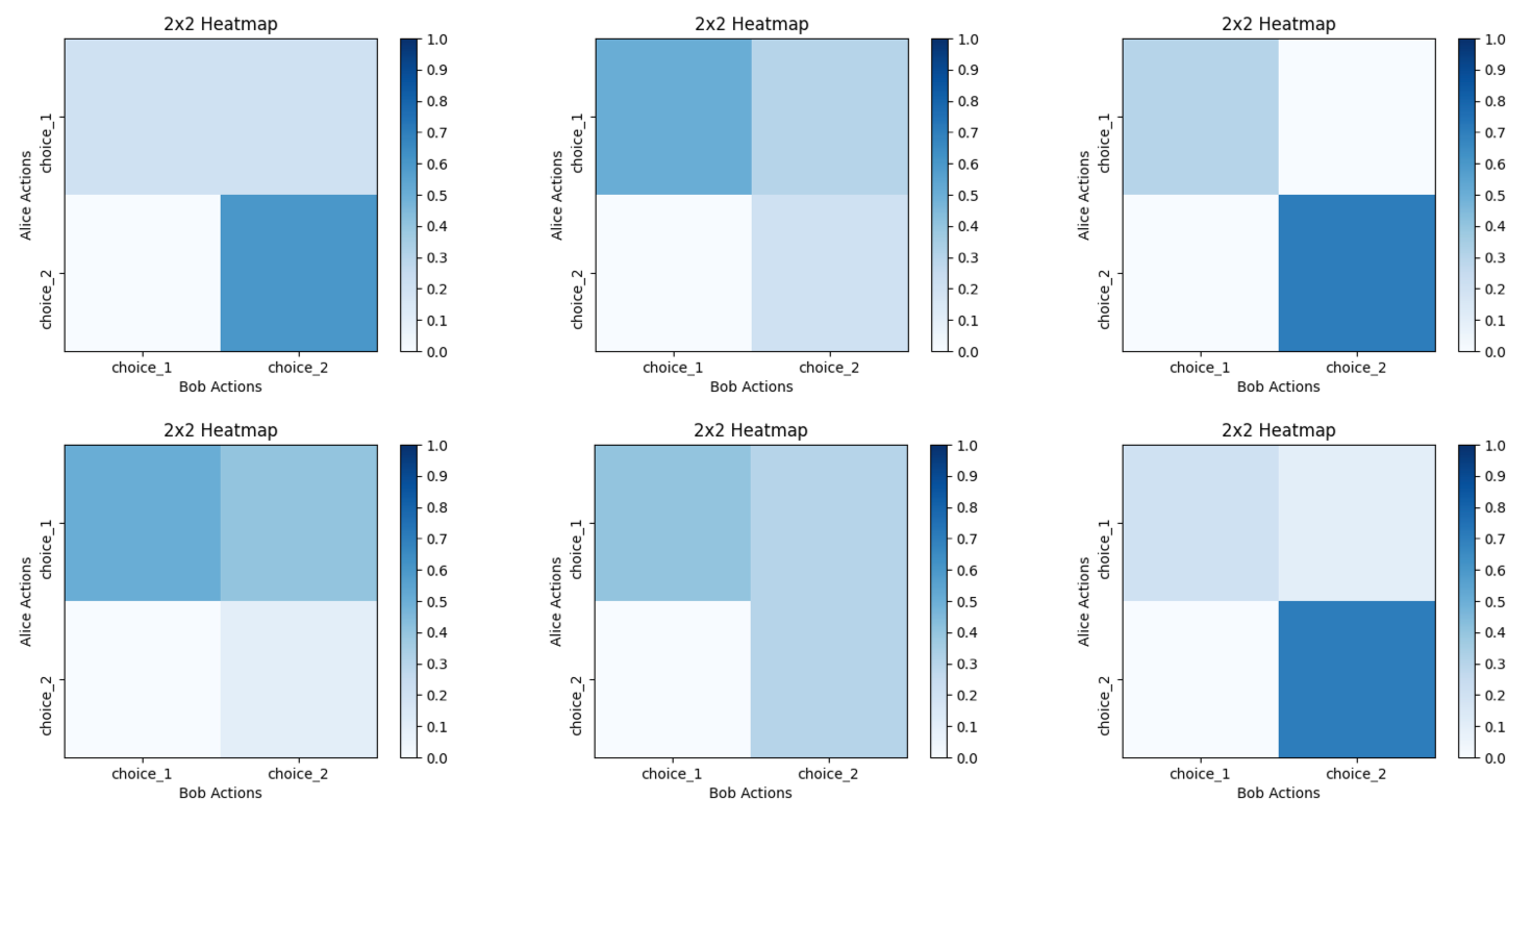
\includegraphics[scale=0.5]{Fig/negotiation_order_bs.pdf}
    \vspace{5pt}\caption{Will the fact that who starts the negotiation affect the result?}
    \label{fig:negotiation_order}
\end{figure}

\subsection{How does the order of negotiation message affect the action?}

It is anticipated that the order in which players initiate negotiations will not influence the final actions taken, particularly in the Battle of the Sexes game. In an ideal scenario, neither the first nor the last player should have a distinct advantage in persuading the other player to act in their favor. To ensure that this is indeed the case, we conduct experiments in the Battle of the Sexes game with varying negotiation rounds (1, 2, and 3) and alter the player who initiates the negotiation, with either player 1 or player 2 starting the negotiation process. This experimental design allows us to investigate the potential impact of negotiation order on the outcomes of the game and assess the fairness of the negotiation process between the two players.

Based on the observation from Figure\ref{fig:negotiation_order}, it is evident that there is no significant change in strategy when the player initiating the negotiation is varied. This observation suggests that the order in which players commence negotiation does not have a substantial impact on the final actions taken in the Battle of the Sexes game. 

\subsection{Irrationality Compared with Humans}
The previous observations suggest that Large Language Models (LLMs) lack robust rationality across various scenarios. However, it is well-established that humans, too, do not always behave rationally \cite{dawes1988anomalies, sally1995conversation}. This raises an intriguing question: do the irrational tendencies of LLMs mirror those of humans?

To investigate this, we adopt a game setting from a televsion game show called Golden Balls where two contestants play a variant on the classic Prisoner's Dilemma: In this game, two players independently decide to either ``split'' or ``steal'' the jackpot. If both choose to split, they share the jackpot equally. If one player chooses to split and the other steals, the stealer takes the entire jackpot. If both players steal, neither receives any money. Human performance of the game is collected by \cite{van2012split}, where players chose to cooperate (i.e., split the jackpot) 53\% of the time on average, a figure consistent with earlier laboratory studies \cite{dawes1988anomalies, sally1995conversation}. The decision to cooperate was sensitive to the size of the jackpot, with cooperation rates decreasing as the stakes increased.

We configured the LLMs to play this game, using the same jackpot sizes as in the human data. Each jackpot size was tested 20 times, resulting in 40 decision-making instances for each size. We then calculated the cooperation rates for the LLMs for different jackpot sizes.

\begin{figure}[!ht]
    \centering
    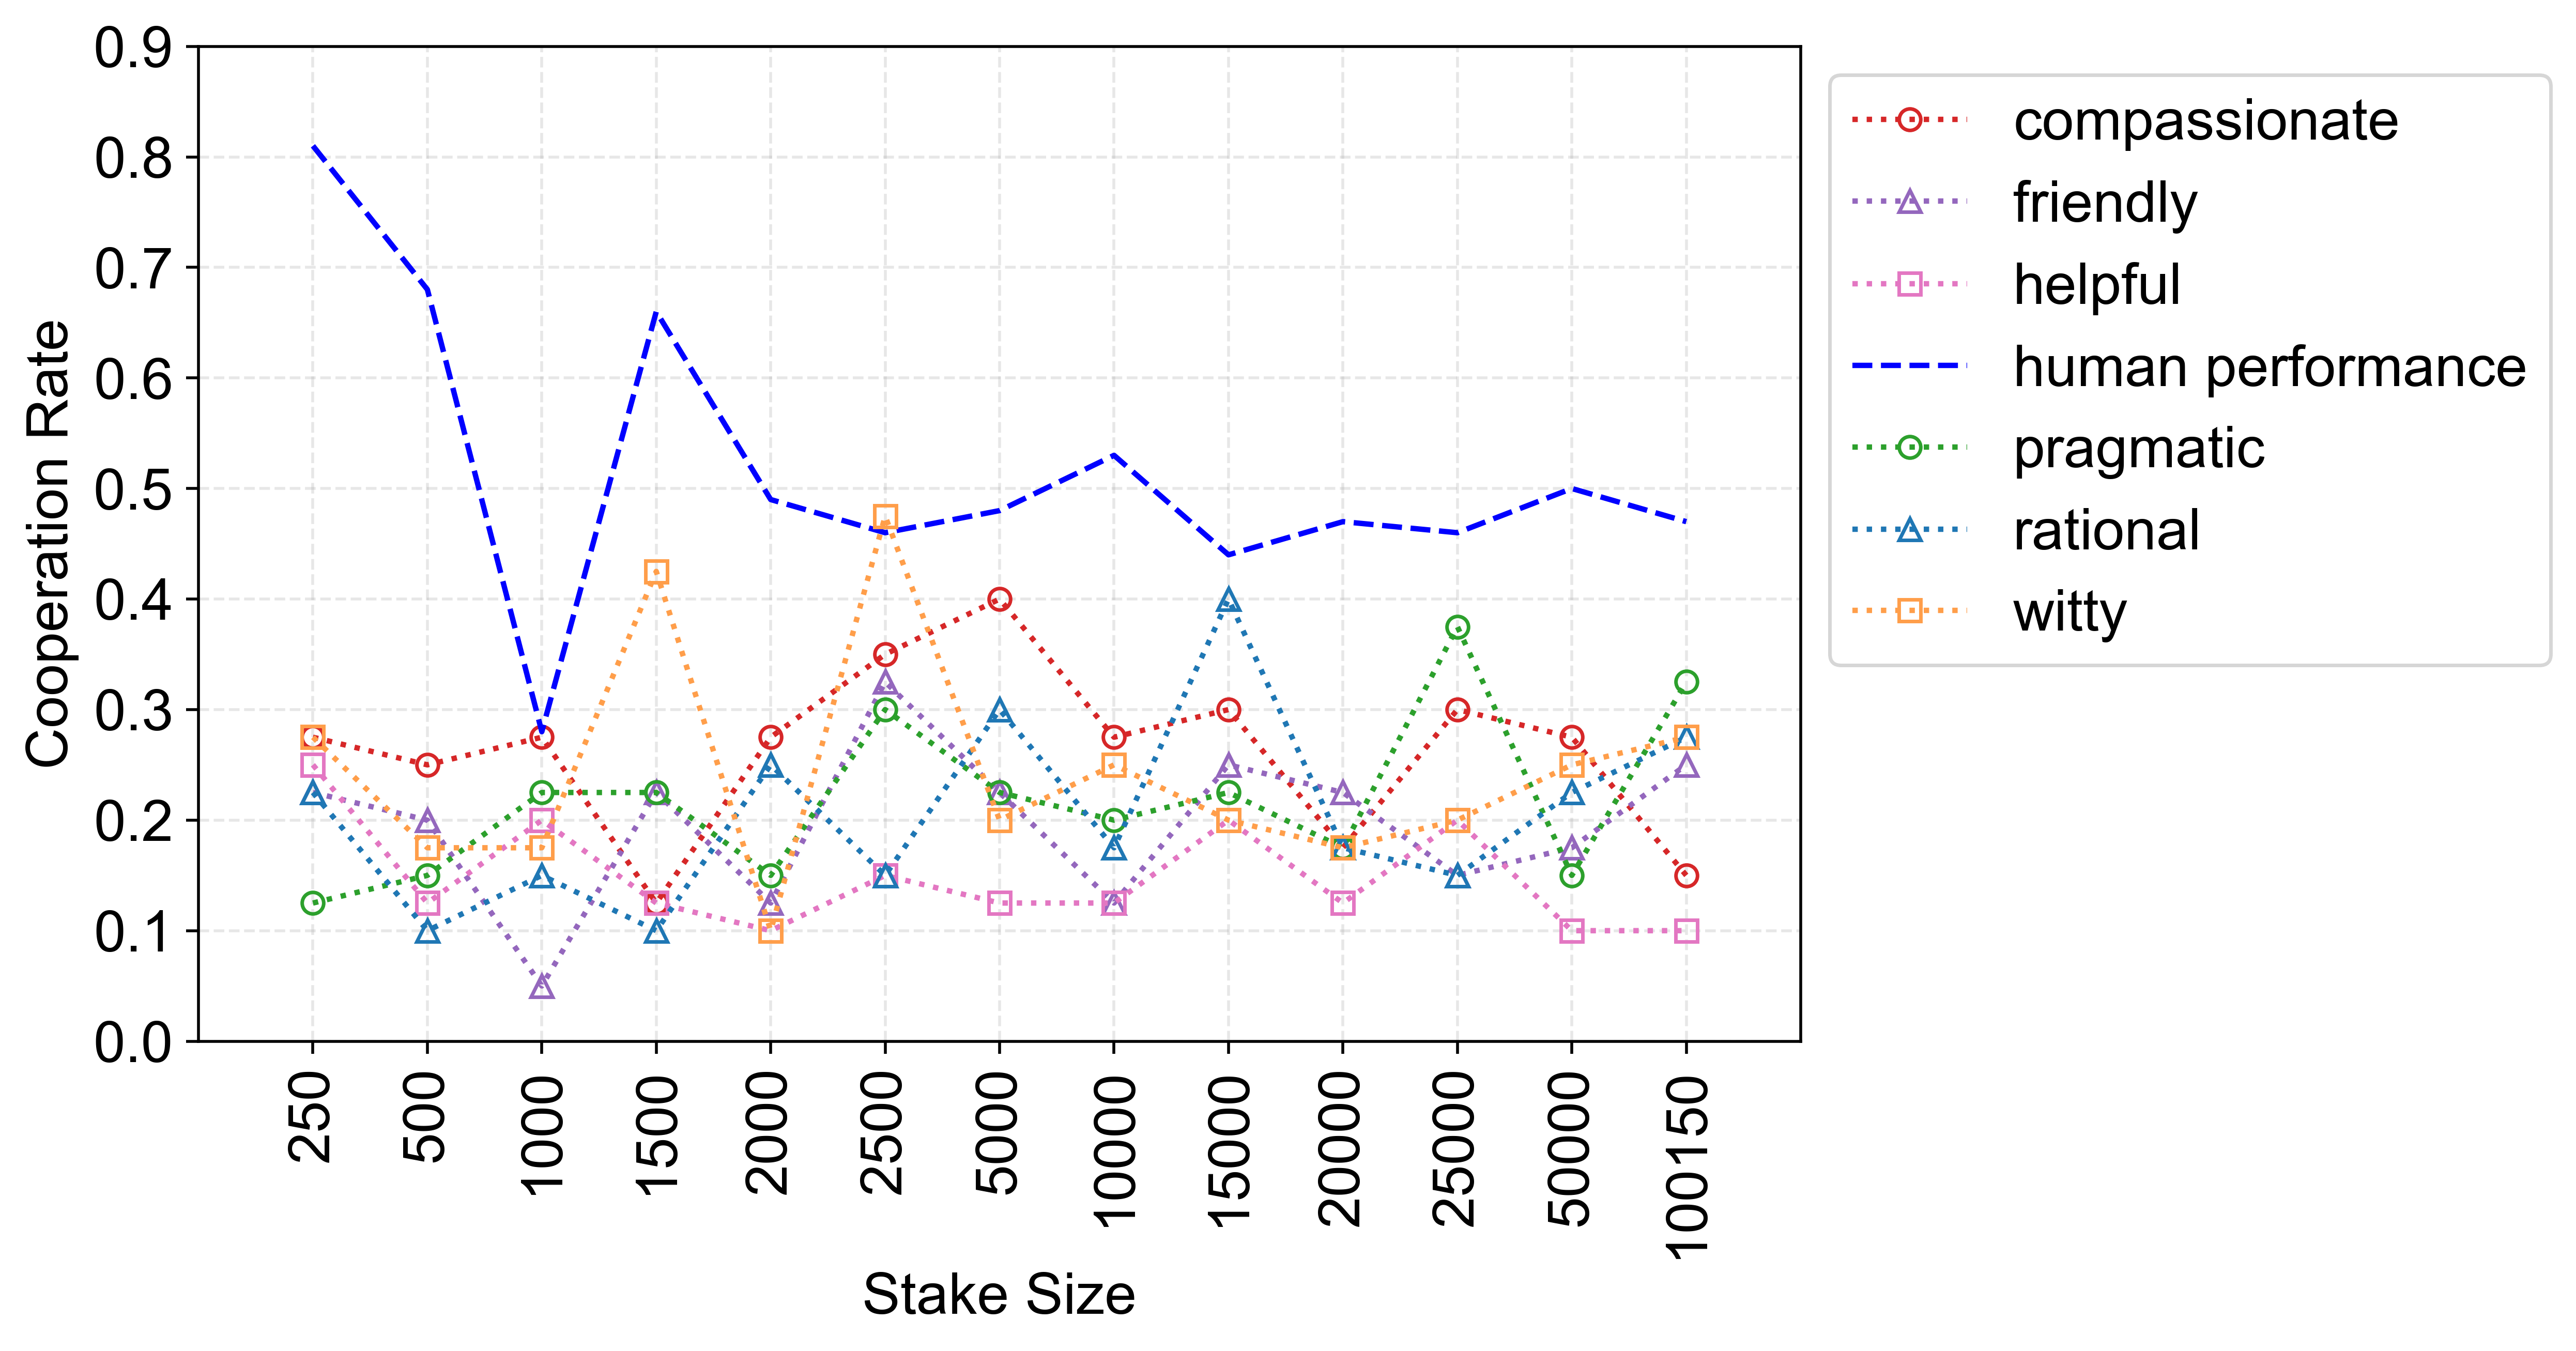
\includegraphics[scale=0.08]{Fig/golden_game.jpg}
    \vspace{5pt}\caption{Rationality analysis on Golden Balls game}
    \label{fig:golden_ball}
\end{figure}

The results of this comparative analysis are presented in Figure~\ref{fig:golden_ball}. Human cooperation rates were indeed sensitive to the size of the jackpot, with higher cooperation rates for smaller jackpots. This trend is also observed in \cite{post2008deal}. In contrast, the LLMs' decision to cooperate was largely insensitive to the jackpot size, regardless of the ``personality'' prompt used: rational, witty, pragmatic, helpful, friendly, compassionate. Furthermore, the LLMs' cooperation rates were generally lower than those of the humans.

While this analysis provides a preliminary comparison of irrational tendencies in LLMs and humans, it is by no means exhaustive. Further research is needed to establish a more comprehensive understanding of the relationship between human and LLM irrationality. 

\begin{minipage}[t]{1\linewidth} 
\begin{tcolorbox}[colback=gray!5,colframe=blue!40!black,title=Summary for raw-LLM v. workflow-LLM and workflow-LLM v. raw-LLM]
\begin{itemize} 
\item \textbf{Lack of Robustness to Numerical Variations}: Empirical results indicate that LLMs either do not exhibit rationality or their rationality is highly sensitive to numerical changes. When the payoff matrix undergoes perturbations that leave the Nash Equilibrium unchanged, the performance of LLMs varies significantly.
\item \textbf{Impact of Negotiation on Rationality}: Consistent with observations made in Section \ref{sec:observation}, we find that rational choices are undermined by the introduction of negotiation, even in the absence of grounds or guarantees for trust.
\item \textbf{Effect of Prompt Variation on Negotiation Impact}: The wording of the prompt can mitigate the influence of negotiation on rationality; however, this mitigating effect diminishes as the number of negotiation rounds increases.
\item \textbf{Order of Negotiation Initiation}: The sequence in which players initiate negotiation does not significantly affect the game's outcome, even in coordination games such as the Battle of the Sexes.
\item \textbf{Comparison of Irrationality Between LLMs and Humans}: Although LLMs lack robust rationality across various scenarios, the nature of their irrationality differs from that observed in human decision-making.
\end{itemize}
\end{tcolorbox} 
\end{minipage}
